\documentclass[10pt]{ctexart}
\usepackage{mypackages}
%\usepackage[UTF8]{ctex} 

\renewcommand{\contentsname}{\erhao\songti{\textbf{目\quad 录}}}
\setcounter{tocdepth}{2}
%\titlecontents{chapter}[0em]{\vspace{3pt}\xiaosi\song\bf}%
%{\prechaptername\CJKnumber{\thecontentslabel}\postchaptername\quad}{} %
%{\hspace{.5em}\titlerule*[7pt]{.}\xiaosi\contentspage}
%\titlecontents{section}[2em]{\vspace{3pt}\xiaosi\song} %
%{\thecontentslabel\quad}{} %
%{\hspace{.5em}\titlerule*[7pt]{.}\xiaosi\contentspage}
%\titlecontents{subsection}[4em]{\vspace{3pt}\xiaosi\song} %
%{\thecontentslabel\quad}{} %
%{\hspace{.5em}\titlerule*[7pt]{.}\xiaosi\contentspage}
%\renewcommand{\bibname}{参考文献}


\begin{document}
    \begin{titlepage}
        \vspace*{-2cm}
        \flushleft
        
\includegraphics[width=0.7\textwidth]{figs/CUGB_fig}\\
        \vspace{3.5cm}
        \begin{center}
            \textbf{\lishu\yihao XXXX课程\\[5pt]结课论文}
        \end{center}
        \vspace{3cm}
        \begin{center}
            \erhao \heiti \parbox[t]{12em}%
            {题目: 这里是你的论文题目}
        \end{center}
        \vspace{2cm}
        \begin{center}
            \songti\sihao
            \renewcommand\arraystretch{1.5}
            \begin{tabular}{p{2cm}c}
                \makebox[2em][l]{学\qquad 院:} & \underline{\makebox[15em][c]{XX学院}} \\
                \makebox[2em][l]{班\qquad 级:} & \underline{\makebox[15em][c]{10XXXXXX}} \\
                \makebox[2em][l]{学\qquad 号:} & \underline{\makebox[15em][c]{10XXXXXXXX}} \\
                \makebox[2em][l]{姓\qquad 名:} &
                \underline{\makebox[15em][c]{XXX}}\\
                \makebox[2em][l]{导\qquad 师:} &
                \underline{\makebox[15em][c]{XXX}}\\
                \makebox[2em][l]{成\qquad 绩:} & \underline{\makebox[15em][c]{ }} \\
                \makebox[2em][l]{时\qquad 间:} & \underline{\makebox[15em][c]{\today}} \\
            \end{tabular}
            
            \vspace{3cm}
            
        \end{center}
    \end{titlepage}
    
    
    
    
    
    \xiaosihao
    \tableofcontents%设置目录
    \thispagestyle{empty}
    \clearpage
    \bibliographystyle{unsrt}
    \setcounter{page}{1}
    
    
    \newpage
    
    
    \textbf{\heiti 摘要:} 本文从实际出发。
    
    
    \textbf{\heiti 关键词:} 1,2,3
    
\section{引言}
    

    % TODO: \usepackage{graphicx} required
    \begin{figure}[H]
        \centering
        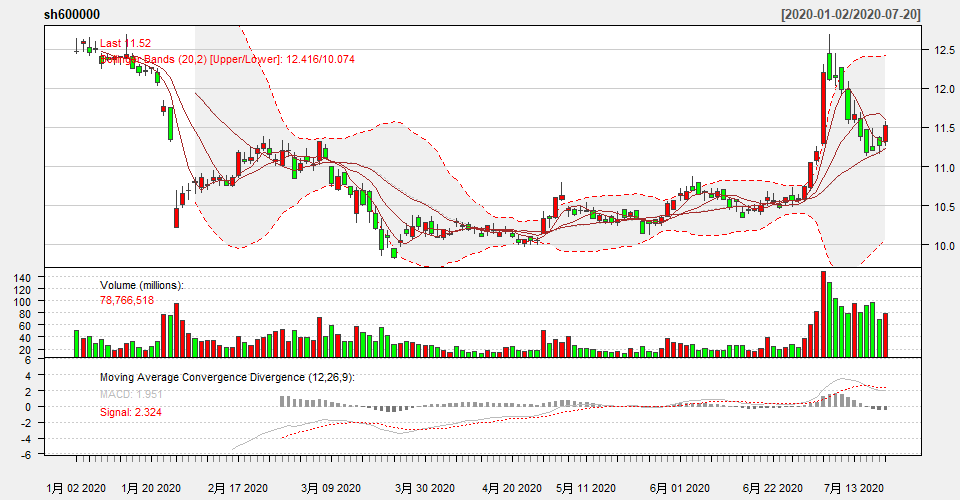
\includegraphics[width=0.95\linewidth]{figs/1}
        \caption[图1]{图形样例}
        \label{fig:1}
    \end{figure}
    
    
\section{总结与体会}
    
    
\begin{thebibliography}{1}        
        
\bibitem{1}
R.~I.Kabacoff.
\newblock {\em R语言实战(第2版)}.
\newblock 人民邮电出版社, 2016.


\end{thebibliography}
    
    
    \section{附录}
    
    \subsection{源代码}


    
    
\end{document}